\begin{figure}[h]
    \centering
    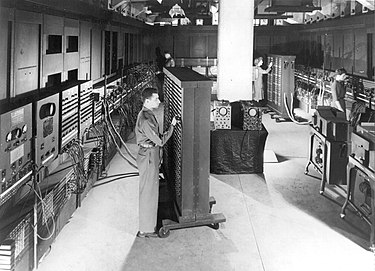
\includegraphics[scale=0.6]{ENIAC_IMG}
    \caption{Mesin ENIAC}
    \label{fig:ENIAC_IMG}
\end{figure}

Komputer di generasi ini ditandai dengan penggunaan tabung vakum di dalam sistemnya.
Salah satu komputer yang termasuk dalam generasi ini adalah komputer ENIAC, atau
\textit{Electronic Numerical Integrator and Computer} ciptaan Amerika Serikat.

Dirancang dan dibuat pada 1945 untuk menjawab berbagai masalah matematis,
ENIAC juga merupakan komputer elektronik \textit{general purpose} atau
komputer umum yang pertama, dan juga merupakan komputer pertama yang dapat diprogram.

ENIAC menggunakan tabung vakum sebagai elemen utama dalam pemrosesannya.
Tabung-tabung vakum tersebut menggantikan sistem relay elektromagnetik yang digunakan
di sistem pendahulunya.

Tabung-tabung vakum digunakan sebagai sebuah ``saklar`` yaitu untuk menyimapan nilai
menyala atau mati (1 atau 0 secara biner). Hingga dengan jumlah yg tepat, tabung-tabung
tersebut dapat mengerjakan operasi-operasi yang cukup rumit, seperti
logika boolean, operasi aritmatika, pemrosesan pararel, dan lain sebagainya.
